% !TEX encoding = UTF-8 Unicode

\documentclass[a4paper]{article}

\usepackage{color}
\usepackage{url}
\usepackage[T2A]{fontenc} % enable Cyrillic fonts
\usepackage[utf8]{inputenc} % make weird characters work
\usepackage{graphicx}
\usepackage[font=small,labelfont=bf]{caption}

\usepackage[english,serbian]{babel}
%\usepackage[english,serbianc]{babel} %uključiti babel sa ovim opcijama, umesto gornjim, ukoliko se koristi ćirilića

\usepackage[unicode]{hyperref}
\hypersetup{colorlinks,citecolor=green,filecolor=green,linkcolor=blue,urlcolor=blue}

%\newtheorem{primer}{Primer}[section] %ćirilični primer
\newtheorem{primer}{Primer}[section]

\begin{document}

\title{3D štampa\\ \small{Seminarski rad u okviru kursa\\Tehničko i naučno pisanje\\ Matematički fakultet}}


\author{    Nevena Miletić\\ mi22193@alas.matf.bf.ac.rs
        \and Matija Todorović\\ mi22282@alas.matf.bf.ac.rs
        \and Đorđe Sajić\\ mi22237@alas.matf.bf.ac.rs
        \and Relja Gajić\\ mi22131@alas.matf.bf.ac.rs
 }

\date{10.novembar 2022.}
\maketitle
\abstract{
        U ovom radu pokušaćemo da vam približimo pojam 3D štampe kao moderne tehnologije za proizvodnju trodimenzionalnih objekata. 3D štampa predstavlja generalno brže, jeftinije i lakše rešenje od drugih tehnologija proizvodnje 3D objekata. U nastavku teksta predstavićemo vam njen razvoj kroz istoriju, tehnike štampanja, kao i primenu u različitim industrijama. }
\tableofcontents

\newpage

\section{Uvod\cite{b}}
\label{sec:uvod}
3D štampa je zapravo aditivna proizvodnja\footnote{Aditivna proizvodnja (eng. \emph{
Additive Manufacturing AM}) predstavlja način proizvodnje gde se iz digitalnog modela
stvara trodimenzionalan predmet}, odnosno proces u kome se slojevi materijala dodaju
jedan na drugi. Kako to zapravo izgleda, videćemo u nastavku.
\bigbreak
3D štampa može da se zamisli kao štampa tankih horizontalnih slojeva. Ti slojevi
predstavljaju horizontalni presek predmeta. Proizvodi koji se dobijaju ovim procesom
mogu biti od različitih materijala. Velikom ekspanzijom 3D štampe, uvode se i novi
materijali, pa je omogućeno istovremeno uklapanje različitih vrsta materijala. Ova
tehnologija proizvodi modele koji mogu da oponašaju izgled i funkcionalnost prototipa.
U poslednjih nekoliko godina cene 3D štampača su sve niže, i samim tim su postali
dostupniji manjim preduzećima, na taj način izrada prototipa se ne zadržava samo u
teškoj industriji. Vremenom mogućnosti koje ovi uredjaji pružaju polako postaju
neograničene.
\bigbreak Tehnologija je nastala 80-ih godina prošlog veka i koristila se pre svega za
proizvodnju prototipova. Ipak, od tada 3D štampa počinje da se koristi kao tehnika za
stvaranje proizvoda gotovo u svim industrijama. Osim izrade prototipa, 3D štampači
nude veliki potencijal za proizvodnju različitih aplikacija u oblasti proizvodnje nakita,
obuće, industrijskog dizajna, arhitekture, automobilske industrije, avio, stomatološke i
medicinske industrije.

\section{Istorija razvoja 3D štampe \cite{c}}

\bigbreak Istorijski gledano, razvoj tehnologije počinje početkom 1980-ih godina. Godine
1981, Hideo Kodama\footnote{Hideo Kodama(1876-1947) – japanski političar i ratni
ministar} prvi je objavio račun o tome kako se materijali koji se nazivaju fotopolimeri
koji su ojačani prilikom izlaganja UV zračenju mogu iskoristiti za brzu izradu čvrstih
prototipa. Iako je on postavio temelje za 3D štampu, on nije napravio prvi 3D štampač.
Te zasluge uzeo je Chuck Hull \footnote{Chuck Hull(1939-)–američki pronalazač}, koji

je dizajnirao i napravio prvi 3D štampač 1984. godine. On je radio za kompaniju koja je
koristila UV lampe za oblikovanje čvrstih, izdržljivih premaza za stolove. Tada dobija
ideju da iskoristi ultraljubičastu tehnologiju za izradu malih prototipa.
\bigbreak Ključ za izradu takvog štampača bili su fotopolimeri koji su ostali u tečnom
stanju sve dok nisu reagovali na ultraljubičastu svetlost. Sistem koji je Hull na kraju
razvio, poznat kao je stereolitografija, koristio je UV zračenje kako bi skicirao oblik
objekta iz kadra tečnih fotopolimera.
\bigbreak On je patentirao tehnologiju 1984. godine, ali tri nedelje nakon što je tim
francuskih pronalazača podneo patent za sličan proces. Međutim, njihovi poslodavci
odlucili su da prestanu da dalje razvijaju tehnologiju zbog"nedostatka poslovne
perspektive". To je omogućilo Hull-u autorsko pravo na pojmam"Stereolithography".
Njegov patent, naslovljen"Aparat za proizvodnju trodimenzionalnih objekata
stereolitografijom" objavljen je u martu 1986. godine.
\bigbreak Dok je Hullov patent obuhvatao mnoge aspekte 3D štampanja, uključujući
dizajn i operativni softver, tehnike i razne materijale, drugi izumitelji bi se nadovezali na
koncept sa različitim pristupima. Tako je 1989. godine dodeljen patent Carlu
Deckardu\footnote{Carl Deckard(1961- )–američki pronalazač, učitelj, diplomant
Univerziteta u Teksasu i biznismen}, koji je razvio metod pod nazivom selektivno
lasersko sinterovanje. Sa SLS-om, laserski zrak se koristi za prilagođavanje praškastih
materijala, kako bi se formirao sloj objekta. Svježi prah bi se dodao na površinu nakon
svakog uzastopnog sloja. Ostale varijacije kao što su direktno metalno lasersko
sinterovanje i selektivno lasersko topljenje se takođe koriste za izradu metalnih predmeta.
\bigbreak Najpopularniji i najprepoznatljiviji oblik 3D štampanja naziva se modeliranje
spojenih depozita. FDP, koji je razvio pronalazač S. Scott Crump\footnote{Scott Crump
(1954- )– pronalazač FDM tehnologije}, postavlja materijal u slojeve direktno na platformu.
Materijal, obično smola, se isprazni kroz metalnu žicu i, nakon puštanja kroz mlaznicu,
odmah se ojača. Ideju za to, Crump je dobio 1988. godine, dok je pokušavao da napravi
igračku žabu za svoju ćerku pomoću voska za sveće i pištolja za lepak.
\bigbreak 1989. godine Crump je patentirao tehnologiju i sa svojom suprugom osnovao
Stratasys Ltd. za proizvodnju i prodaju 3D štamparskih mašina za brzo prototipiranje ili
komercijalnu proizvodnju.
Kompaniju su izveli u javnost 1994. godine, a do 2003. godine FDP je postao
najprodavanija tehnologija brže prototipizacije.

\section{Tehnike 3D štampe\cite{c}}
\label{sec:naslov1}
Prema tehnici 3D štampanja možemo razlikovati sledeće tehnologije:
\begin{itemize}
\item \textbf{Inkjet}
\item \textbf{Fused Deposition Modelin(FDM)}
\item \textbf{Stereolitografija}
\item \textbf{Selektivno lasersko sinterovanje (SLS)}
\item \textbf{Proizvodnja objekata laminacijom (LOM)}
\end{itemize} 



 


\subsection{Inkjet}
\label{subsec:podnaslov1}
Ubrizgavanje (eng. \emph{Inkjet}) - kreira prototip na osnovu 3D modela tako što pravi sloj po sloj projekta.
\bigbreak Ističe se po atributu da je prilagodljiv na razne oblike tečnih materijala što pruža stvaranje konduktivnih ili izolacionih struktura u visokoj rezoluciji što dovodi do lakšeg implementiranja kompleksnih oblika. 
\bigbreak Za razliku od drugih procesa, injekt štampanju nije potrebno dodatno prerađivanje i obrada nako izvršenog štampanja.
\bigbreak Prilikom izrade materijali u tečnom stanju se stavljaju na vrh za štampanje (eng. Printing head) koji pravi dati projekat.
\bigbreak Kao što slika 1 prikazuje uz glavni materijal, koji se koristi za izradu modela,  se može dodati pomoćni materijal (eng. Support material) koji mu daje čvrstinu i stabilnost prilikom izrade.
\begin{center}
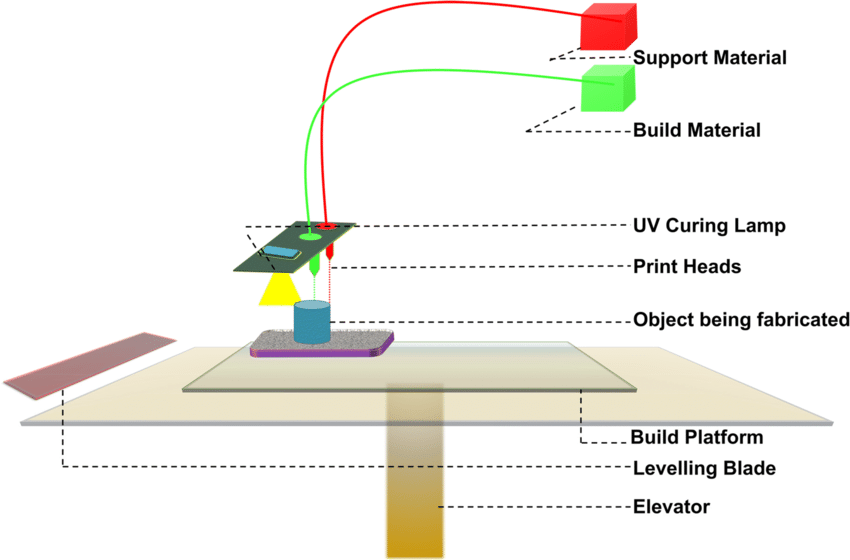
\includegraphics[width=.5\textwidth ]{Tehnikeslike/Inject.png}
\captionof{figure}{Model ubrizgavanja (eng. \emph{Inkjet}) }
\end{center}

\subsection{Fused Deposition Modelin(FDM)\cite{fdm}}
\label{subsec:podnaslov2}
FDM (eng. \emph{Fused Deposition Modeling}) - predstavlja najkorišćenu i najjeftiniju tehniku za 3D štampanje. Lak je za korišćenje, on koristi termoplastične filamente \footnote{Termoplastični filament - materijali za 3D štampanje od termoplastičnih polimera. Oni se oblikuju prilikom zagrevanja. } sa ektruzijom između svakog sloja.
\bigbreak Najčešće se koristi u developovanju proizvoda  i test modela koji inžinjeri koriste da provere da li oblik odgovara datom uređaju po dimenzijama. 
\bigbreak Sastoji se od podloge na kojoj se izvršava štampanje, displeja za štampanje, mašine koja zagreva filamente i kulera koji održava temperaturu uređaja.

\begin{center}
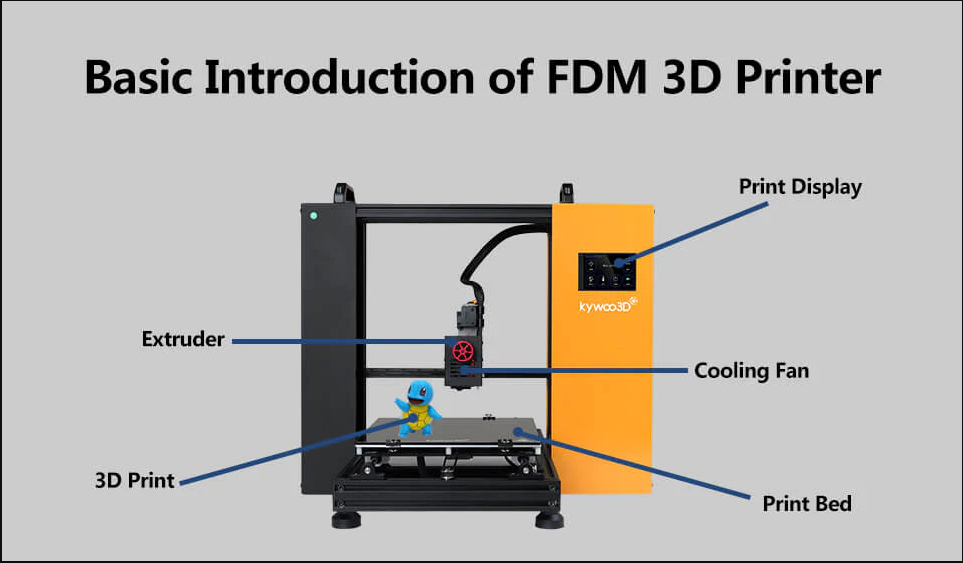
\includegraphics[width=.5\textwidth ]{Tehnikeslike/FDM.PNG}
\captionof{figure}{Uprošćena šema FMD 3D štampača }
\end{center}

\subsection{Stereolitografija}
\label{subsec:podnaslov3}
Stereolitografija (eng. \emph{Stereolithography SLA}) - Koristi rezervoar tečnog fotopolimera\footnote{Fotopolimer - polimer koji ima različite hemijske reakcije u zavisnosti od temperature.}  koji formira sloj po sloj projekta, gde se nakon formiranja svakog sloja polimer stvrdne uz pomoć ultraljubičastog svetla.
\bigbreak Nakon svakog odrađenog sloja podloga se spušta kako bi krenula obradu sledećeg. Kada se završi obrada 3D modela potrebno je izvršeni projekat oprati rastvaračem da bi se uklonila tečnost opasna po život.
\bigbreak Ova tehnika se najčešće koristi za kreiranje 3D modela visokih rezolucija.  Stereolitografija koristi pomoćne stubove koji sprečavaju da dođe do deformacije prilikom izgradnje sledećih slojeva koji se nalaze iznad njega.


\begin{center}
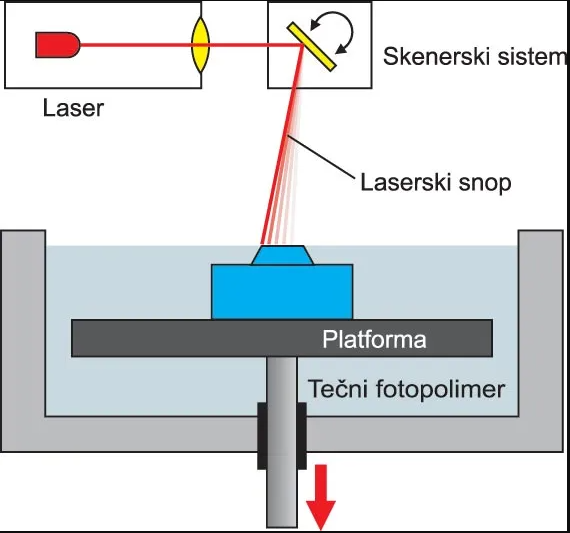
\includegraphics[width=.5\textwidth ]{Tehnikeslike/Stereolitografija.PNG}
\captionof{figure}{Šema stereolitografije}
\end{center}

\bigbreak
\bigbreak

\subsection{Selektivno lasersko sinterovanje (SLS)\cite{e}}
\label{subsec:podnaslov4}
Izborno lasersko lemljenje (eng. \emph{Selective Laser Sintering SLS}) - koristi se za pravljenje prototipa od metala i plastike. Uz pomoć zrna materijala (eng. \emph{powder beds}) mašina pravi dizajne sloj po sloj, pri čemu koristi lasersko grejanje i zbijanje (sinterovanje) praha datog materijala. 
\bigbreak Nakon svakog sloja postolje se spušta i dodaje novi sloj materijala sve dok mašina ne završi izgradnju modela. Pošto čvrstina modela zavisi od najveće temperature mašine SLS zagreje prevremeno prah materijala ispod njengove temperature topljenja kako bi dostigao maksimalne temperature za najmanji period, što isto omogućava da laser lakše izreže željene oblike za sloj. 
\bigbreak Kao što je pokazano na slici 4 rezervoari (eng. \emph{powder tank}) stavljaju prah na vrh prethodnog sloja, dok se njegova platforma spušta za sledeći sloj.
\bigbreak Sečivo za slojeve (eng. \emph{recoater blade}) prolazi i ravna vrh modela, nakon toga laser gradi i oblikuje dati model. 
\begin{center}
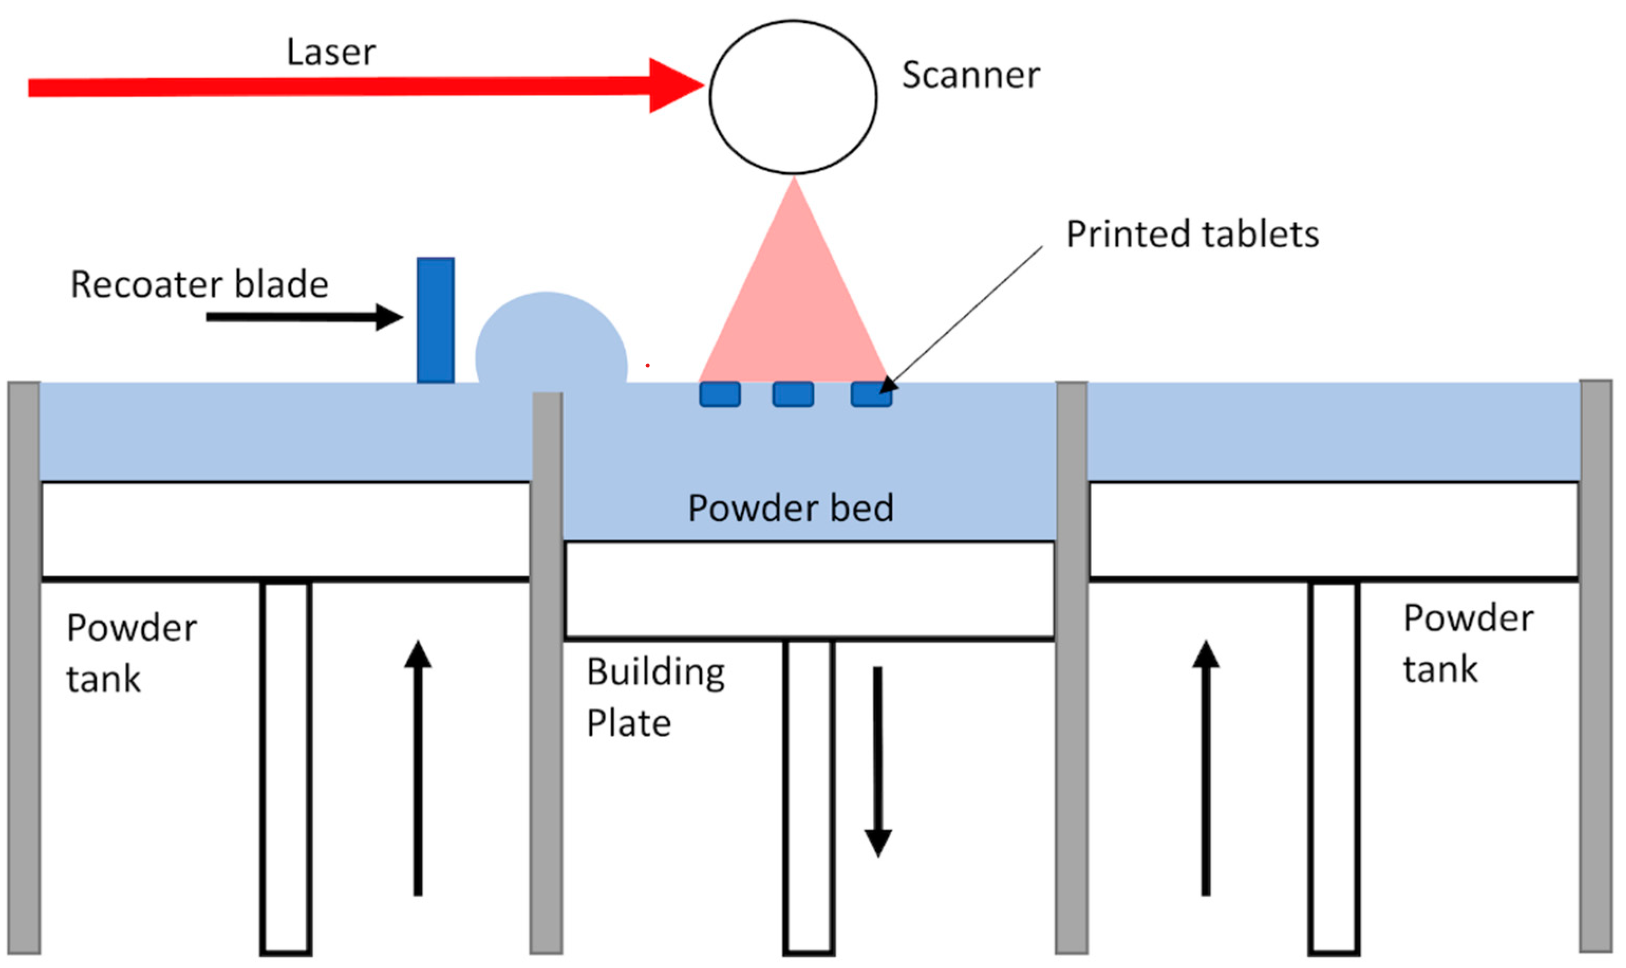
\includegraphics[width=.5\textwidth ]{Tehnikeslike/Sls.png}
\captionof{figure}{Šema SLS-a}
\end{center}
\newpage
\subsection{Proizvodnja objekata laminacijom (LOM)\cite{lom}}
\label{subsec:podnaslov5}
Proizvodnja objekata laminacijom (eng. \emph{ Laminated object manufacturing LOM}) - Korišćenjem papira premazanim lepkom, plastiku ili metalni laminat kao sredstvo za 3D štampanje. 
\bigbreak Hartije se lepe jedna za drugu sloj po sloj na platformi uz pomoć motora koji na krajevima imaju rolne korišćenog materijala (eng. \emph{Material spool}).
\bigbreak Na radnoj površini se seku u željeni oblik pomoću noža ili lasera, a neiskorišćeni ostatak ide u rolnu koja se nalazi u smeru obrtanja motora.
\bigbreak Nakon tog procesa projekat se može doraditi šmirglanjem i bušenjem ako je potrebno.

\begin{center}
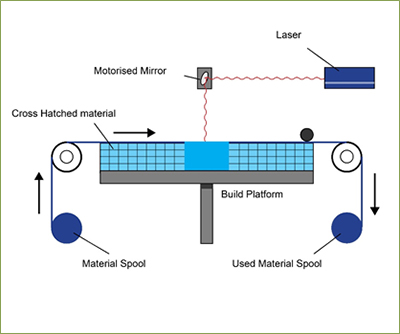
\includegraphics[width=.5\textwidth ]{Tehnikeslike/LOM.jpg}
\captionof{figure}{Šema LOM-a}
\end{center}

\begin{center}
\begin{tabular}{||c c c ||} 
 \hline
 Broj & Tip  & Materijali \\ [1ex] 
 \hline\hline
 1 & tečni materijali  &\\ 
 \hline
 2 & FDM & termoplastični filamenti \\
 \hline
 3 & SLA & tečni fotopolimer\\
 \hline
 4 & SLS & metal ili plastika\\
 \hline
 5 & LOM & papir premazan lepkom, plastiku ili metalni laminat\\ [1ex] 
 \hline
\end{tabular}
\captionof{table}{Tipovi - Materijal} 
\end{center}

\newpage

\section{Primena\cite{a}}
\label{sec:Primena}

U proteklih nekoliko godina, štampači postaju sve dostupniji i dostupniji. Više se ne koriste isključivo u teškoj industriji, već i u manjim preduzećima i čak i za ličnu upotrebu. Koriste se u najrazličitije svrhe i skoro svim granama privrede. Kao što je već napomenuto, broj raznovrsnih materijala koji se koriste za rad sa 3d štampačima je ogroman i raste vrtoglavom brzinom. To omogućava veliku raznovrsnost njihove primene. 

\subsection{Medicina}
\label{subsec:podnaslov6}

Primena 3D štampača u medicini je počela 2014. godine u Velikoj Britaniji kada je pacijentu koji je od posledica raka izgubio gotovo pola kože lica, upravo putem 3D štampe napravljen novi deo lica i postavljen na mesto starog. Ovo predstavlja veliki korak u modernoj medicini jer se prvi put dogodilo da je čovek u mogućnosti da odštampa neki deo svog tela. 
\bigbreak Ovakvi procesi se izvršavaju primenom fotogrametrije. Proces se sastoji iz niza kamera koje prave fotografije zdravih tkiva pacijenta, a zatim ga računarski sklapaju u jednu 3D celinu koja će kasnije biti odštampana. Proces slikanja i izrade celine je vrlo brz i traje svega nekoliko sati, dok je proces štampanja vrlo delikatan i sa veoma malim prostorom za grešku, naravno, traje znatno duže od prethodnih. Pričvršćivanje novog, štampanog tkiva se izvršava hirurškim zahvatom.

\subsection{Prototipovi}
\label{subsec:podnaslov7}

Ovo je najvažniji i najrasprostranjeniji vid primene 3D štampača. Dizajnerima je znatno olakšan i ubrzan rad. Štampač može uz korišćenje male količine materijala i u kratkom vremenskom roku da stvori prototip za čiju bi izradu bilo potrebno značajno više. Ovaj vid primene se koristi u gotovo svim granama privrede.

\subsection{Vojna primena}
\label{subsec:podnaslov8}

Naravno, ljudi su vrlo brzo našli primenu 3d štampačima u vojnoj industriji. Konkretno, za izradu delova za pištolje i puške, kao i za izradu bojeve municije. Počelo je tako što je jedan mladi amerikanac došao na ideju da napravi jeftine delove za svoju pušku, što mu je i pošlo za rukom. Ono što je izuzetno privlačno kompanijama za proizvodnju oružja, kao i vladama i organizacijama koje ga kupuju, je upravo mogućnost pravljenja oružja kome se ne može ući u trag. U vojnoj industriji se očekuje najveći porast primene štampača. 

\subsection{Izrada odeće i obuće}
\label{subsec:podnaslov9}

Razne kompanije za proizvodnju odeće i obuće obilato koriste 3D štampače. Ne toliko za pravljenje konkretnih celina kao što su patike, već za pravljenje raznih manjih delova. Poznati su upravo delovi za sportsku odeću poput krampona za kopačke ili ojačanih vrhova pertli.

\section{Zaključak}
\label{sec:Zaključak}

U proteklih nekoliko godina, primena kao i dostupnost 3D štampanja raste, 3D štampa prelazi iz sveta fikcije u realan svet i uskoro ce se pretopiti u savremenu upotrebu. Od krucijalne važnosti je dalji razvitak ove tehnologije jer su, teorijski, mogućnosti neograničene i trenutno je jedini limit nivo tehnologije našeg vremena. 3D štampanje će moći imati ogroman udeo u raznim sferama kao što su medicinske svrhe, inženjering, avio i automobilske industrije...
\newpage
 
%\addcontentsline{toc}{section}{Literatura}
%\appendix

%\iffalse
%\bibliography{seminarski} 
%\bibliographystyle{plain}
%\fi

%\begin{thebibliography}{9}

%\bibitem{cryptography} Gary C. Kessler. \emph{https://3dstampa.rs/sta-je-3d-stampa/}, 2015.

%\bibitem{Diffie-Hellman} Maryam Ahmed, Baharan Sanjabi, et al. \emph{https://3dstampa.rs/sta-sve-moze-da-se-3d-stampa/}, (IJESIT), 2012.

%\bibitem{use} David A. Carts. \emph{https://bs.eferrit.com/ko-je-pronasao-3d-stampanje/}, SANS Institute, 2001.

%\bibitem{logjam} Adrian, David; et al. (October 2015). \emph{https://www.rapiddirect.com/blog/3d-prototyping/}

%\bibitem{pohlig-hellman} Mollin, Richard (2006-09-18). \emph{An Introduction To Cryptography} (2nd ed.). Chapman and Hall/CRC. p. 344

%\bibitem{dhstandard} E. Rescorla (June 1999). \emph{https://www.nano-di.com/resources/blog/2019-the-3d-inkjet-printing-process-explained}

%\bibitem{dlproblem} Kevin S. McCurley (1990). \emph{https://www.twi-global.com/technical-knowledge/faqs/what-is-laminated-object-manufacturing-lom}

%\bibitem{ddh-vs-cdh} A. Joux, K. Nguyen (2003). \emph{https://tractus3d.com/knowledge/learn-3d-printing/fdm-3d-printing/}

%bibitem{dhpaper} J. F. Raymond, A. Stiglic (2000). \emph{Security Issues in the Diffie-Hellman Key Agreement Protocol}

%\bibitem{elgamal} T.Elgamal (1985). \emph{A public key cryptosystem and a signature scheme based on discrete logarithms}

%bibitem{rb} L. Batina, J. Daemen (2021). \emph{Diffie-Hellman key agreement and ElGamal encryption}

%\end{thebibliography}

%https://3dstampa.rs/sta-je-3d-stampa/
%https://3dstampa.rs/sta-sve-moze-da-se-3d-stampa/
%https://bs.eferrit.com/ko-je-pronasao-3d-stampanje/
%https://www.rapiddirect.com/blog/3d-prototyping/
%https://www.nano-di.com/resources/blog/2019-the-3d-inkjet-printing-process-explained
%https://www.twi-global.com/technical-knowledge/bifaqs/what-is-laminated-object-manufacturing-lom
%https://tractus3d.com/knowledge/learn-3d-printing/fdm-3d-printing/
\bibliographystyle{plain}
\bibliography{19_MileticTodorovicGajicSajic.bib}
\end{document}
